\documentclass[12pt,a4paper]{article}
\usepackage[polish]{babel}
\usepackage[T1]{fontenc}
\usepackage{lmodern}
\usepackage[utf8x]{inputenc}
\usepackage{hyperref}
\usepackage{url}
\usepackage{graphicx}
\usepackage{listings}
%\usepackage{xcolor}
\usepackage{color}
\usepackage{float}
\usepackage{multicol}
\usepackage{tikz}
\usepackage{makecell}
% FOREST
\usepackage[edges]{forest}

\definecolor{foldercolor}{RGB}{124,166,198}

\tikzset{pics/folder/.style={code={%
    \node[inner sep=0pt, minimum size=#1](-foldericon){};
    \node[folder style, inner sep=0pt, minimum width=0.3*#1, minimum height=0.6*#1, above right, xshift=0.05*#1] at (-foldericon.west){};
    \node[folder style, inner sep=0pt, minimum size=#1] at (-foldericon.center){};}
    },
    pics/folder/.default={20pt},
    folder style/.style={draw=foldercolor!80!black,top color=foldercolor!40,bottom color=foldercolor}
}

\forestset{is file/.style={edge path'/.expanded={%
        ([xshift=\forestregister{folder indent}]!u.parent anchor) |- (.child anchor)},
        inner sep=1pt},
    this folder size/.style={edge path'/.expanded={%
        ([xshift=\forestregister{folder indent}]!u.parent anchor) |- (.child anchor) pic[solid]{folder=#1}}, inner ysep=0.6*#1},
    folder tree indent/.style={before computing xy={l=#1}},
    folder icons/.style={folder, this folder size=#1, folder tree indent=3*#1},
    folder icons/.default={12pt},
}

% SETTINGS
\addtolength{\hoffset}{-1.5cm}
\addtolength{\marginparwidth}{-1.5cm}
\addtolength{\textwidth}{3cm}
\addtolength{\voffset}{-1cm}
\addtolength{\textheight}{2.5cm}
\setlength{\topmargin}{0cm}
\setlength{\headheight}{0cm}
\renewcommand{\arraystretch}{1.5}

\title{Academic Data Deliverer\\Programowanie Obiektowe i Graficzne}
\author{Artur Bednarczyk, Dawid Grajewski, Damian Kwaśniok\\Politechnika Śląska\\Wydział Matematyki Stosowanej\\Informatyka, semestr IV}
\date{\today}

\begin{document}
	\maketitle
	\begin{figure}[H]
		\centering
		\includegraphics[width=0.5\linewidth]{LOGO2}
		\label{fig:logo}
	\end{figure}
	\clearpage
	\tableofcontents
	\clearpage
	\section{Harmonogram prac}
	\begin{tabular}{|p{0.7\textwidth}|c|c|}
	\hline
	Co & Kto & Kiedy \\	\hline\hline
	Projekt bazy danych & Bednarczyk & 04.2018 \\ \hline
	Utworzenie bazy danych & Grajewski & 04.2018 \\ \hline
	Połączenie z bazą danych & Grajewski & 10.05.2018 \\ \hline
	Projekty graficzne & Bednarczyk & 13.05.2018 \\ \hline
	\makecell[l]{Szkielet struktury MVP \\
	Wyśrodkowanie widoku z możliwością rozszerzenia okna} & Bednarczyk & 23.05.2018 \\ \hline
	Logowanie & Kwaśniok & 26.05.2018 \\ \hline
	Sesja i Hash & Grajewski & 26.05.2018 \\ \hline
	Przełączanie między widokami & Grajewski & 28.05.2018 \\ \hline
	\makecell[l]{Wyświetlanie listy notatek\\
	Wyświetlanie notatki\\
	Zapis notatki do pliku\\
	Wyświetlanie danych użytkownika w profilu\\
	Wyświetlanie listy subskrybowanych kierunków w profilu}& Bednarczyk & 31.05.2018 \\ \hline
	Rejestracja & Kwaśniok & 31.05.2018\\ \hline
	Dodawanie i anulowanie subskrypcji dla kierunku & Bednarczyk & 02.06.2018 \\ \hline
	Testowanie i poprawki & \makecell{Bednarczyk \\Grajewski \\Kwaśniok} & 03.06.2018 \\ \hline
	\hline
	Dokumentacja & \makecell{Bednarczyk} & Cały czas\\ \hline
	\end{tabular}
	\clearpage
	\section{Opis projektu}
		\subsection{Opis}
			Aplikacja dla studentów umożliwiająca szybki i łatwy podgląd dostępnych materiałów! Każdy student może wybrać kierunki studiów, którymi jest zainteresowany i oglądać przypisane do nich notatki! W każdej chwili  może dodać nowe lub usunąć nieinteresujące go kierunki ze swojej listy. Aplikacja jest prosta w użytkowaniu, jednak wymaga połączenia z internetem.

		\subsection{Projekt UI}
			\subsubsection{Logowanie}
				Obrazek.png
			\subsubsection{Rejestracja}
				Obrazek.png
			\subsubsection{Profil}
				Obrazek.png
			\subsubsection{Notatka}
				Obrazek.png
		\subsection{Funkcjonalności}
			\subsubsection{Logowanie i Rejestracja}
				Załóż swoje konto, a będziesz mógł korzystać z aplikacji z każdego urządzenia, na którym jest zainstalowana i posiada dostęp do internetu! Zachowaj Twoje listy kierunków na swoim koncie!
			\subsubsection{Przypasanie do grup}
				Wybierz kierunki, które Cię interesują i przeglądaj materiały z nimi powiązane. W każdej chwili możesz dopisać do swojej listy nowe kierunki lub usunąć już niepotrzebne.
			\subsubsection{Notatki}
				Przeglądaj dostępne materiały z listy kierunków, którą sam utworzyłeś. Jeśli chcesz mieć dostęp offline to pobierz materiał w formie pliku!
	\section{Technologie}
			\subsection{Oprogramowanie}
			\begin{itemize}
			\item Visual Studio 2015 - Środowisko programistyczne.
			\item SourceTree - Kontrola wersji.
			\item GitHub - Repozytorium do przechowywania wersji online.
			\item Heroku - Chmura, w której przechowywana jest baza danych.
			\end{itemize}
			\subsection{Technologie}
			\begin{itemize}
			\item C\#
			\item .NET
			\item MySQL
			\end{itemize}
			\clearpage
	\section{Implementacja}
		\subsection{Podział projektu na pliki}
		\begin{multicols}{2}
\scalebox{0.9}[0.7]{
			\begin{forest}
				for tree={font=\sffamily, grow'=0,
    folder indent=.3em, folder icons}
    	[ADD
			[.Models	
				[.Interfaces
					[ILoginModel.cs, is file]
					[INoteModel.cs, is file]	
					[IProfileModel.cs, is file]	
					[IRegisterModel.cs, is file]	
					[ISubscribeModel.cs, is file]					
				]
				[.Results
					[Result.cs, is file]				
				]
				[.Session
					[ISession.cs, is file]
					[Session.cs, is file]				
				]  
				[.Utils
					[.Encrypters
						[IEncrypter.cs, is file]
						[SHA1Encrypter.cs, is file]					
					]
				]
				[LoginModel.cs, is file]
				[NoteModel.cs, is file]
				[ProfileModel.cs, is file]
				[RegisterModel.cs, is file]
				[SubscribeModel.cs, is file]
			]
			[.Presenters
				[LoginPresenter.cs, is file]
				[NotePresenter.cs, is file]
				[ProfilePresenter.cs, is file]
				[RegisterPresenter.cs, is file]
				[SubscribePresenter.cs, is file]			
			]
			[.UserControl
				[LoginControl.cs, is file]
				[NoteControl.cs, is file]
				[ProfileControl, is file]
				[RegisterControl, is file]			
			]
			[.Views
				[ILoginControl.cs, is file]
				[INoteControl.cs, is file]
				[IProfileControl, is file]
				[IRegisterControl, is file]			
				[ISubscribeView, is file]
			]
		]
			\end{forest}
}
\scalebox{0.9}[0.7]{			
	        \begin{forest}
				for tree={font=\sffamily, grow'=0,
    folder indent=.3em, folder icons}
    	[DAL
    		[.Models
				[.Entity
					[College.cs, is file]
					[Faculty.cs, is file]
					[Lecturer.cs, is file]
					[Material.cs, is file]
					[Specialization.cs, is file]
					[Subject.cs, is file]
					[User.cs, is file]
					[UserSpecialization.cs, is file]
				]
				[.Repository
					[CollegesRepository.cs, is file]		
					[FacultiesRepository.cs, is file]
					[LecturersRepository.cs, is file]
					[MaterialsRepository.cs, is file]
					[SpecializationsRepository.cs, is file]
					[SubjectsRepository.cs, is file]
					[UsersRepository.cs, is file]
					[UsersSpecializationsRepository.cs, is file]
				]    		
    		]
    	]
    \end{forest}
    }
    \scalebox{0.9}[0.7]{
    \begin{forest}
				for tree={font=\sffamily, grow'=0,
    folder indent=.3em, folder icons}
    	[COMMOM
    		[Logger.cs, is file]
    		[LogType.cs, is file]
	    ]
	        \end{forest}
}
		\end{multicols}	
		\subsection{Schemat Modelu Obiektowego}
			\begin{figure}[H]
			\centering
			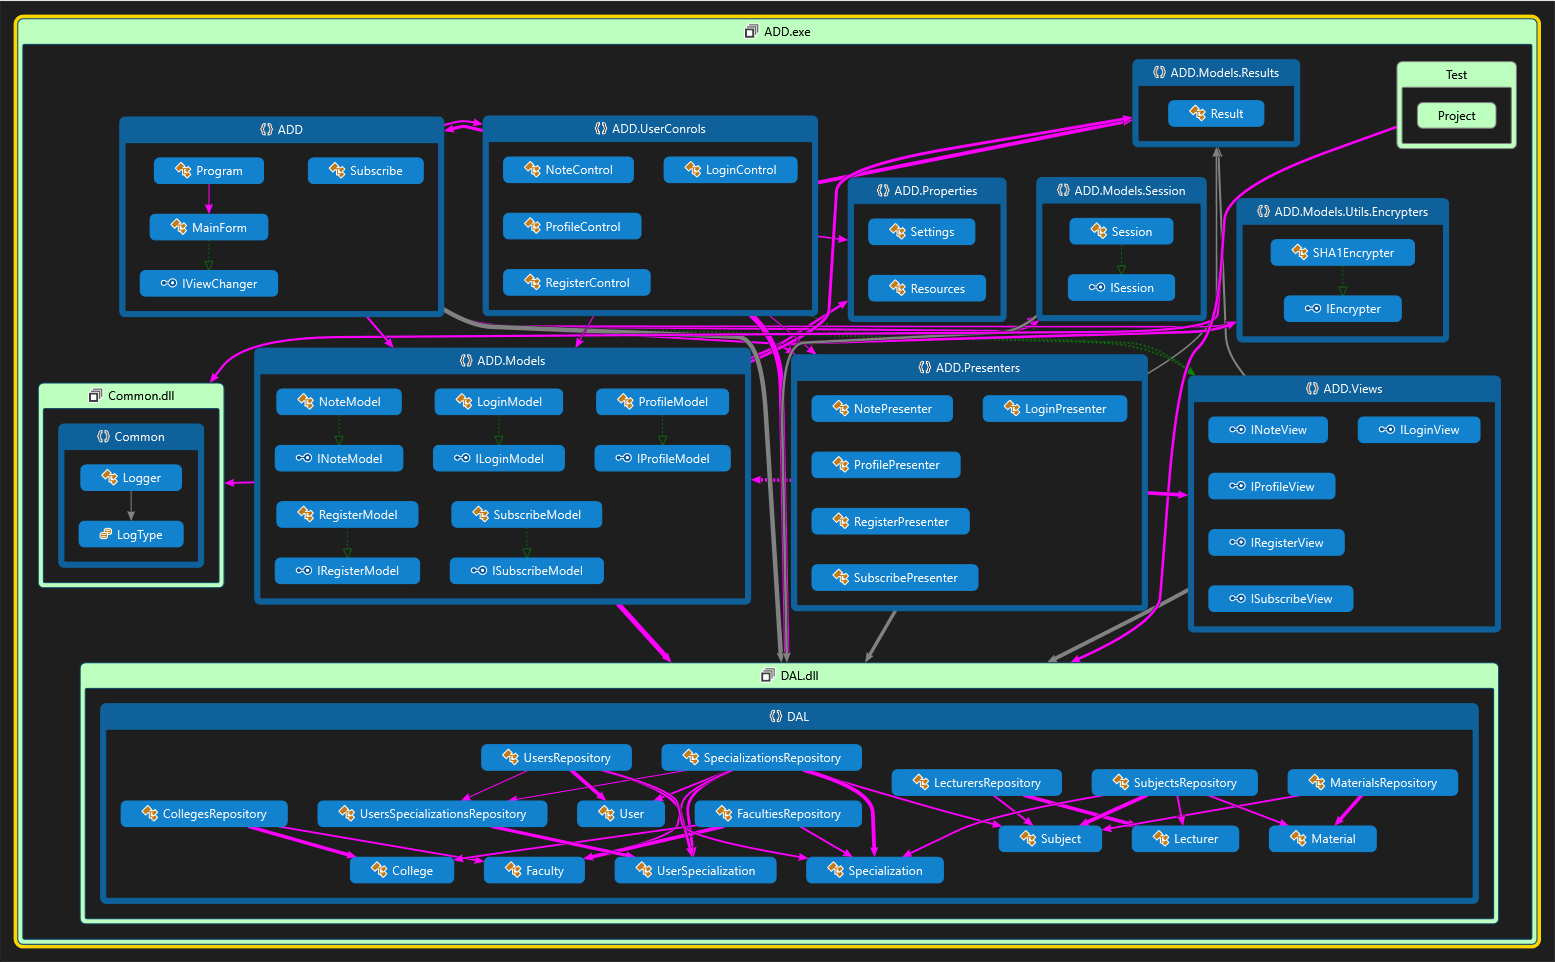
\includegraphics[width=1.0\textwidth]{class_diagram}
			\end{figure}
		\subsection{Interfejsy}
			\begin{itemize}
				\item Models
				\begin{itemize}
					\item ILoginModel - bla bla bla
				\end{itemize}
				\item Views
				\begin{itemize}
					\item ILoginView - bla bla bla
				\end{itemize}
			\end{itemize}
		\subsection{Rozwiązania}
			Wszystkie nasze rozwiązania są tak cudowne, że trzeba by opisać cały kod linijka po linijce <3
	\section{Testy}
		Działa. 
\end{document}